%\documentclass[draft, 12pt]{article}
\documentclass[12pt]{article}
\usepackage[utf8]{inputenc} % следующие две строки используются для
\usepackage[english,russian]{babel}   % руссификации AmSLaTeX
\usepackage{amsmath,amsfonts,amssymb,euscript,graphicx,wrapfig,multirow}
\usepackage{dsfont}
\inputencoding{utf8}
\textheight=240mm \textwidth=170mm
\hoffset=-17mm % сдвиг влево
\voffset=-17mm % сдвиг вверх

\begin{document}

\noindent УДК 511.95 + 514.112

\begin{center}
\textbf{Об отыскании целоудалённых множеств специального вида} \\[3mm]
\textbf{Н.~Н.~Авдеев}\\[2mm]
\emph{ВГУ}
\end{center}

Целоудалённым множеством (ЦМ) будем называть такое подмножество $M$ плоскости $\mathbb{R}^2$,
не содержащееся ни в какой прямой,
что расстояние между любыми двумя точками $M$ есть целое число.

Эрдёш [TODO: ссылки!] доказал, что любое ЦМ конечно.
(Доказательство на русском языке можно найти в [TODO: ссылки!].)

Для ЦМ естественным образом определяется диаметр:
$$
	diam(M) = \max_{A,B\in M} |A-B|,
$$
где $|A-B|$~--- обычное расстояние между $A$ и $B$.

Задача об отыскании ЦМ заданного диаметра и мощности первоначально возникла
в ходе определения минимального диаметра,
которым может обладать множество заданной мощности [TODO: ссылка на первые работы].
Затем, в ходе развития классификации ЦМ и выделения множеств полуобщего и общего положения,
встал вопрос от отыскании ЦМ, обладающих специальными свойствами.


В данной работе описывается отыскание <<необычных>>, в некотором смысле, ЦМ.

Выделяют веерные ЦМ, т.е. ЦМ, лежащие на объединении прямой и некоторой точки.
Именно веерные ЦМ имеют наименьший диаметр среди всех ЦМ мощности от 9 до 122 [TODO: Kurz];
однако с помощью веерных ЦМ невозможно построить конструктивную оценку на минимальный диаметр,
которая была бы существенно лучше, чем существующая [TODO:ссылка], основанная на содержащихся в окружности ЦМ.
С помощью инверсии и растяжения плоскости можно из веерного ЦМ сконструировать ЦМ,
содержащееся в объединении окружности с её центром [TODO: ссылка].
Таким образом, относительно хорошо известны ЦМ, лежащие в объединении точки с прямой или окружности с её центром.
Отыскание таких ЦМ выходит за пределы целей данной работы.

На основе веерного ЦМ характеристики 1 легко строится ЦМ, содержащееся в двух перпендикулярных прямых,
при этом на одной из прямых лежит 2 или 3 точки, на другой~--- все остальные
(точка пересечения прямых может как принадлежать ЦМ, так и не принадлежать ему).
Отыскание ЦМ, содержащихся в паре перпендикулярных прямых и распределённых по этим прямым
<<более равномерно>>, де-факто оказывается чисто алгебраической [TODO:ссылка];
наиболее интересным, на взгляд автора, является следующий пример из [TODO:ссылка]:
$$
TODO:
.
$$

Таким образом, нас будут интересовать все ЦМ, кроме ЦМ, содержащихся:
а) В объединении прямой с точкой, не лежащей на ней (веерные ЦМ);
б) В объединении окружности с её центром;
в) В паре перпендикулярных прямых.

Для отыскания ЦМ используется алгоритм, описанный в [TODO: строяк],
со следующими изменениями.
Во-первых, нахождение ЦМ с заданным диаметром и мощностью не приводит к прекращению процесса поиска.
Во-вторых, в модифицированном алгоритме Брона-Кербоша за начальную клику
принимается не произвольная точка, лежащая за пределами прямой, проходящей через точки,
на которых достигается диаметр, а пара таких точек (если расстояние между точкми пары есть число целое).
Это отсекает значительное количество (но не все) веерных ЦМ.

Все найденные таким алгоритмом ЦМ подвергаются проверке на выполнение одного из условий (а)--(в);
если ни одно из условий не выполнено, информация о ЦМ записывается в файл и строится визуализация найденного ЦМ с помощью gnuplot
[TODO: ссылочку бы].

Ниже приводятся иллюстрированные примеры найденных ЦМ из числа наиболее интересных.
Для облегчения восприятия иногда применяется запись вида
$\sqrt{p}/q * \{ (x_1,y_1), ...,$ $ (x_n, y_n)  \}$,
означающая, что каждую абсциссу нужно умножить на $1/q$,
а каждую ординату~--- умножить на $\sqrt{p}/q$, т.е.
$$
	\sqrt{p}/q * \{ (x_1,y_1), ..., (x_n, y_n)  \}
	=
	\left\{ \left(\frac{x_1}{q},\frac{y_1\sqrt{p}}{q}\right), ..., \left(\frac{x_n}{q},\frac{y_n\sqrt{p}}{q}\right)  \right\}
	.
$$

Чаще всего из интересующих нас ЦМ встречаются ЦМ, содержащиеся в паре параллельных прямых,
причём на одной из прямых лежит две или три точки.

\begin{itemize}
\setlength{\itemsep}{-1mm}


\item
$\sqrt{35}/{34} * \{ (\pm 289, 0),
%(289 , 0),
(88 , -39),
(-144 , -15),
(-175 , 48),
(-57 , -24),
(57 , 24)\} $
(рис.~\ref{Avdeev_7_17_1538484835387.eps}).
%ЦМ мощности 7, диаметр 17.
На этом ЦМ достигается минимальное значение диаметра для мощности 7,
однако в [TODO: ссылка, fig. ] это ЦМ приведено не было:
примером ЦМ мощности 7 и диаметра 17 послужило другое ЦМ.

\item
$\sqrt{3}/2 * \{
( \pm 56 , 0),
( 14 , 0),
( -34 , 0),
( -10 , 24),
( -21 , 35),
( 35 , -21)
\}
$
(рис.~\ref{Avdeev_7_56_1538484851696.eps}).
ЦМ лежит на двух пересекающихся под острым углом прямых и имеет ось симметрии
~--- биссектрису угла между прямыми.


\begin{figure}[htbp]
	\includegraphics[width=.48\linewidth]{Avdeev_7_17_1538484835387.eps}
	\hfill
	\includegraphics[width=.48\linewidth]{Avdeev_7_56_1538484851696.eps}
	\\
	\parbox{.48\linewidth}{\caption{ЦМ мощности 7, диаметр 17}\label{Avdeev_7_17_1538484835387.eps}}
	\hfill
	\parbox{.48\linewidth}{\caption{ЦМ мощности 7, диаметр 56}\label{Avdeev_7_56_1538484851696.eps}}
\end{figure}


\begin{figure}[htbp]
	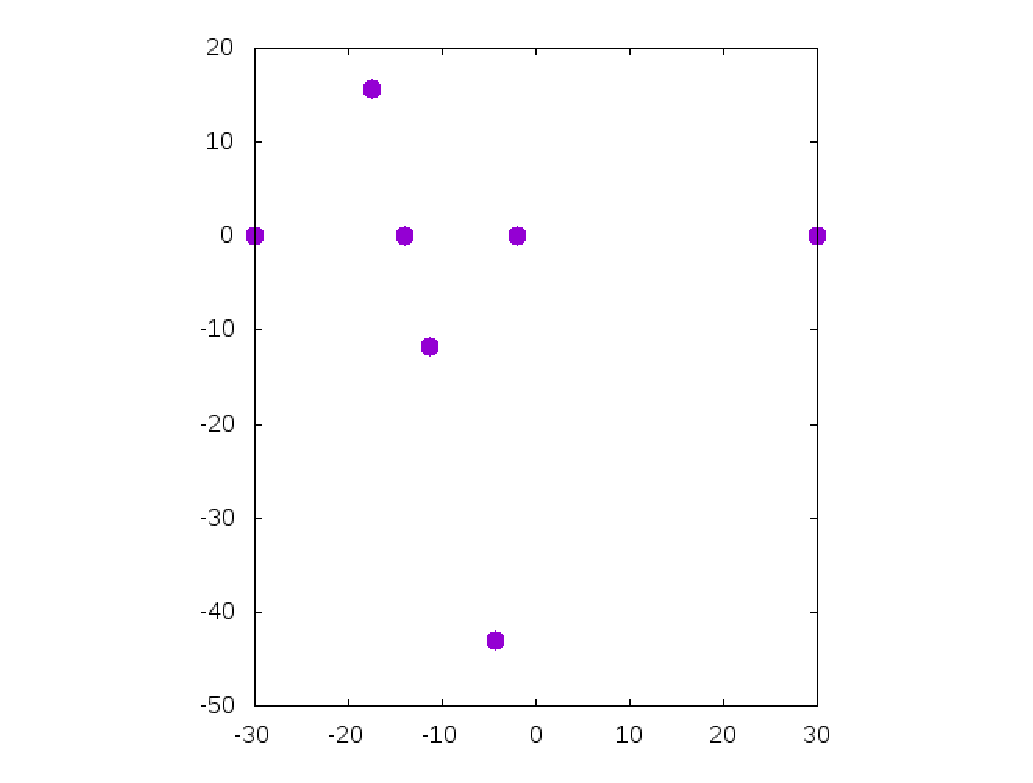
\includegraphics[width=.48\linewidth]{Avdeev_7_60_1538484853808.eps}
	\hfill
	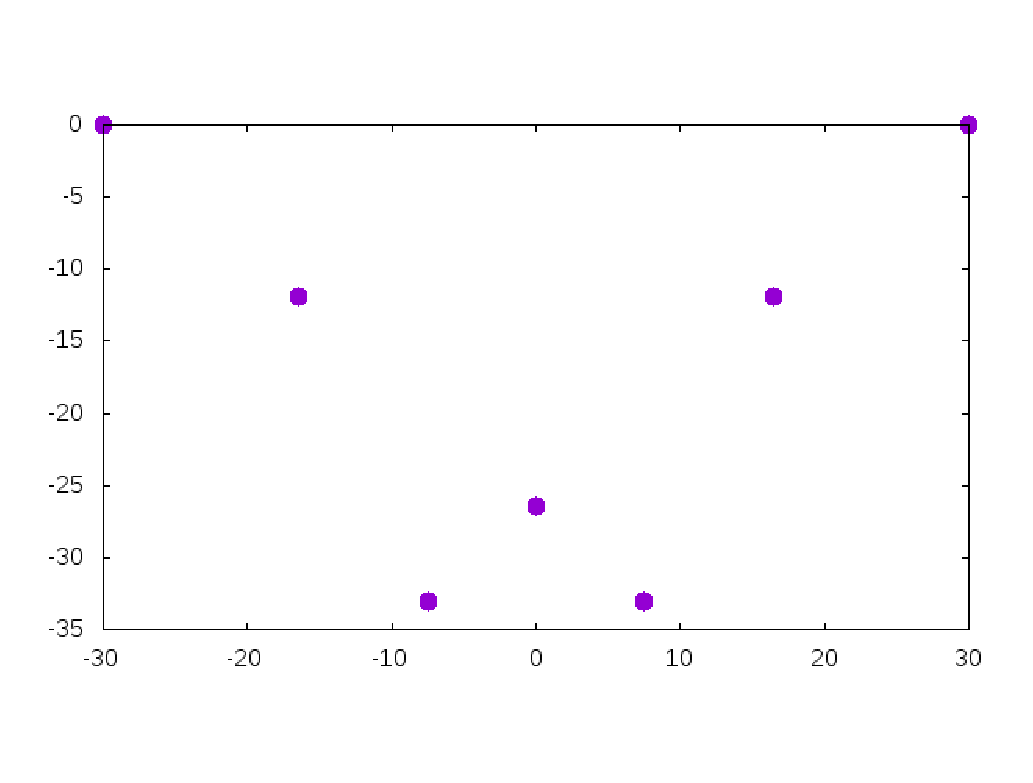
\includegraphics[width=.48\linewidth]{Avdeev_7_60_1538484854748.eps}
	\\
	\parbox{.48\linewidth}{\caption{}\label{Avdeev_7_60_1538484853808.eps}}
	\hfill
	\parbox{.48\linewidth}{\caption{}\label{Avdeev_7_60_1538484854748.eps}}
\end{figure}


\begin{figure}[htbp]
	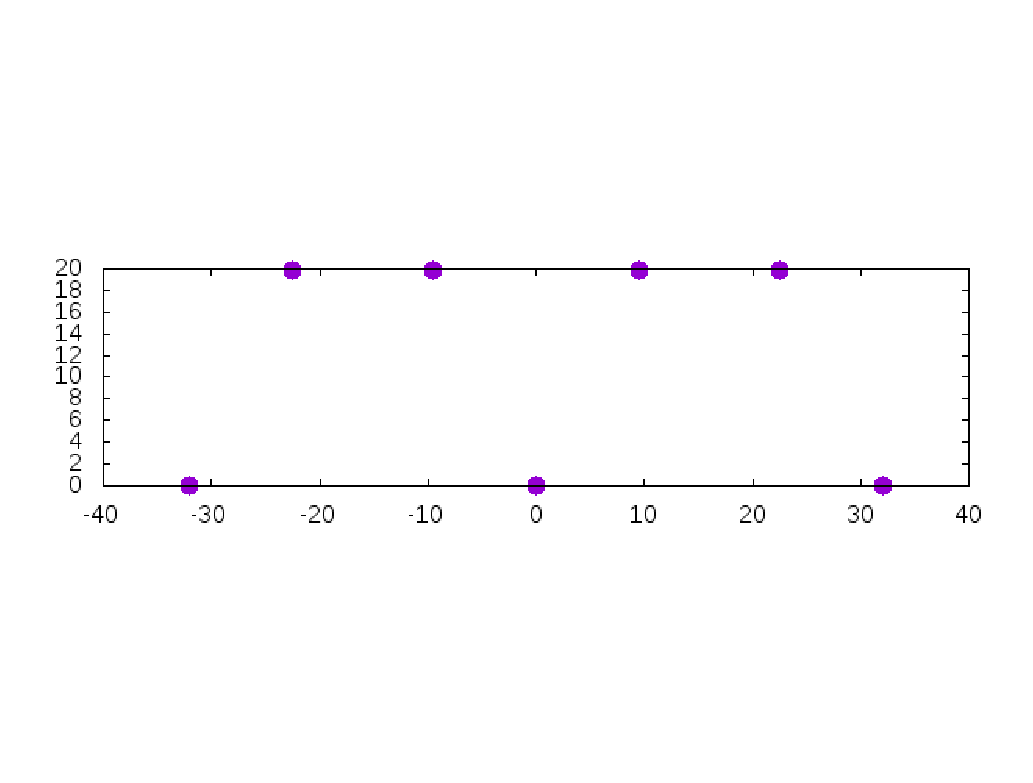
\includegraphics[width=.48\linewidth]{Avdeev_7_64_1538484861024.eps}
	\hfill
	\includegraphics[width=.48\linewidth]{Avdeev_7_75_1538484880810.eps}
	\\
	\parbox{.48\linewidth}{\caption{}\label{Avdeev_7_64_1538484861024.eps}}
	\hfill
	\parbox{.48\linewidth}{\caption{}\label{Avdeev_7_75_1538484880810.eps}}
\end{figure}


\begin{figure}[htbp]
%	\includegraphics[width=.48\linewidth]{}
	\hfill
%	\includegraphics[width=.48\linewidth]{}
	\\
	\parbox{.48\linewidth}{\caption{}\label{}}
	\hfill
	\parbox{.48\linewidth}{\caption{}\label{}}
\end{figure}



\begin{figure}[htbp]
	\includegraphics[width=.48\linewidth]{Avdeev_8_123_1538485378899.eps}
	\hfill
	\includegraphics[width=.48\linewidth]{Avdeev_8_123_1538485378698.eps}
	\\
	\parbox{.48\linewidth}{\caption{}\label{Avdeev_8_123_1538485378899.eps}}
	\hfill
	\parbox{.48\linewidth}{\caption{}\label{Avdeev_8_123_1538485378698.eps}}
\end{figure}



\begin{figure}[htbp]
	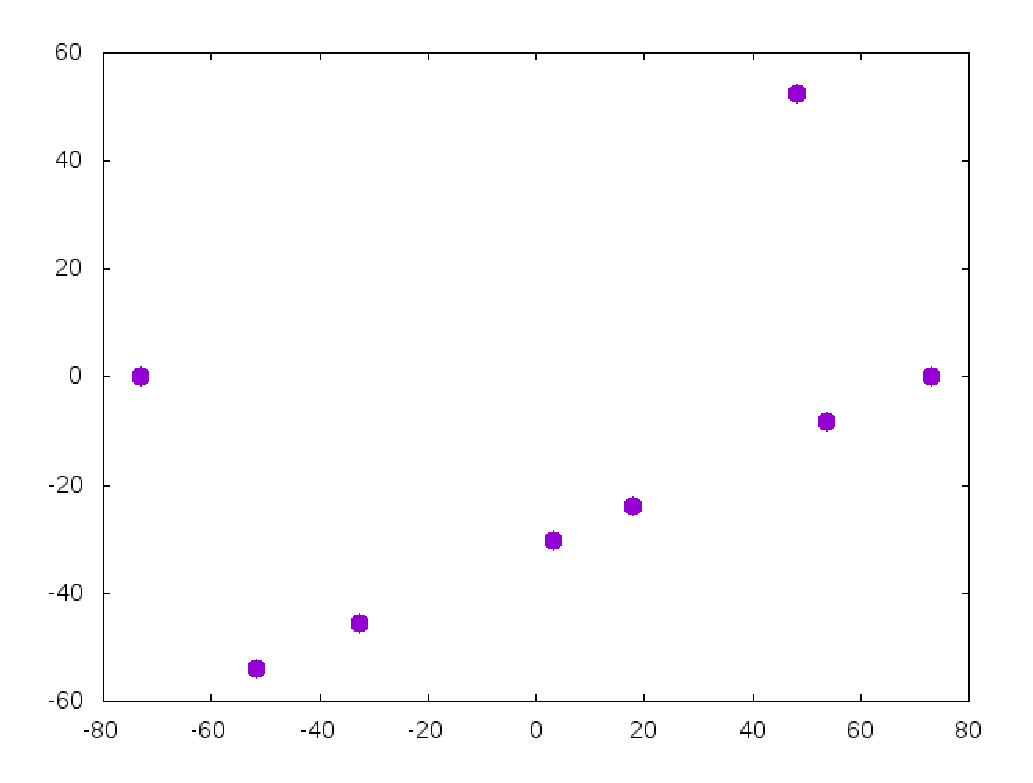
\includegraphics[width=.48\linewidth]{Avdeev_8_146_1538486493354.eps}
	\hfill
	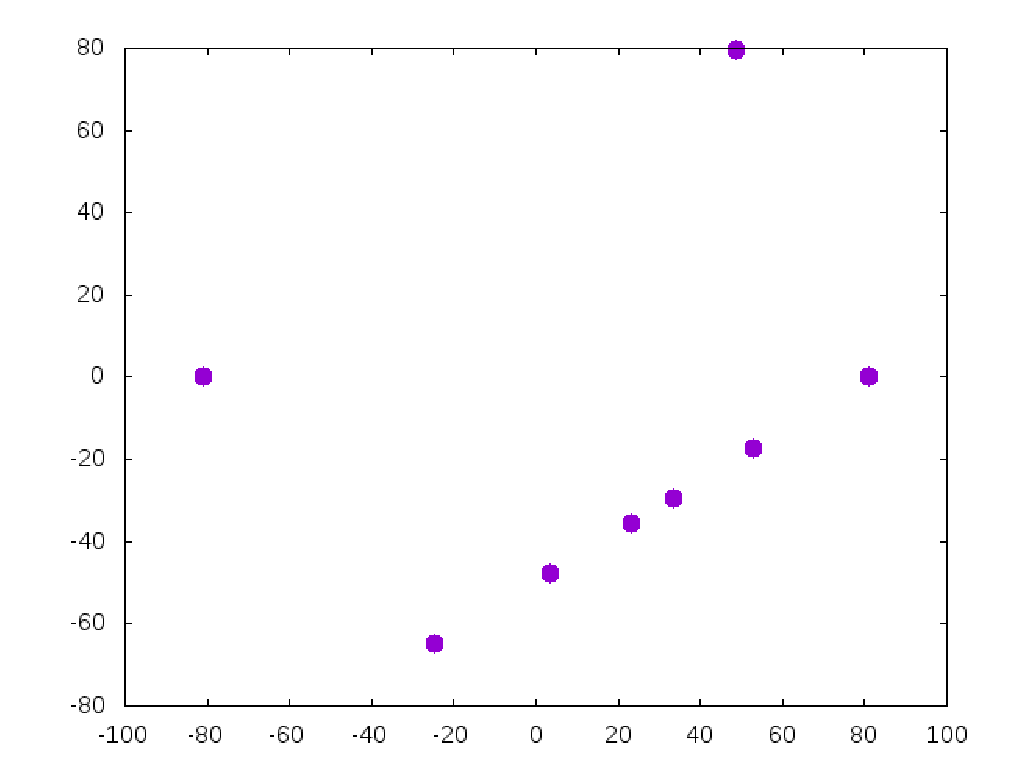
\includegraphics[width=.48\linewidth]{Avdeev_8_162_1538488466583.eps}
	\\
	\parbox{.48\linewidth}{\caption{}\label{Avdeev_8_146_1538486493354.eps}}
	\hfill
	\parbox{.48\linewidth}{\caption{}\label{Avdeev_8_162_1538488466583.eps}}
\end{figure}




\begin{figure}[htbp]
	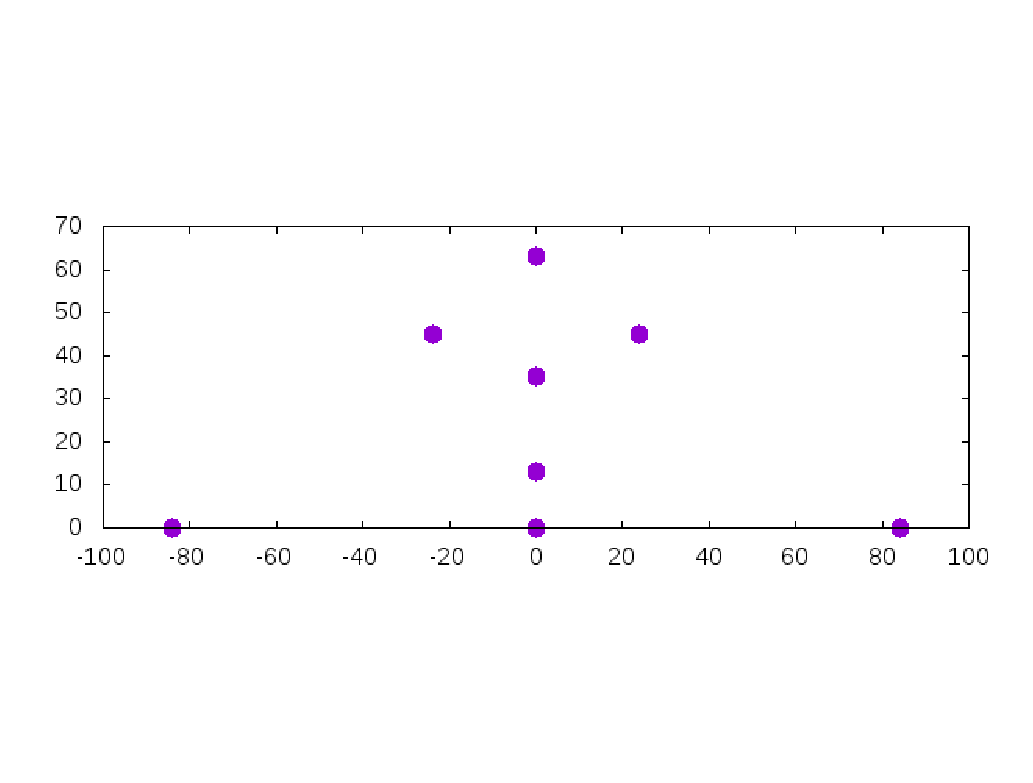
\includegraphics[width=.48\linewidth]{Avdeev_8_168_1538490487450.eps}
	\hfill
	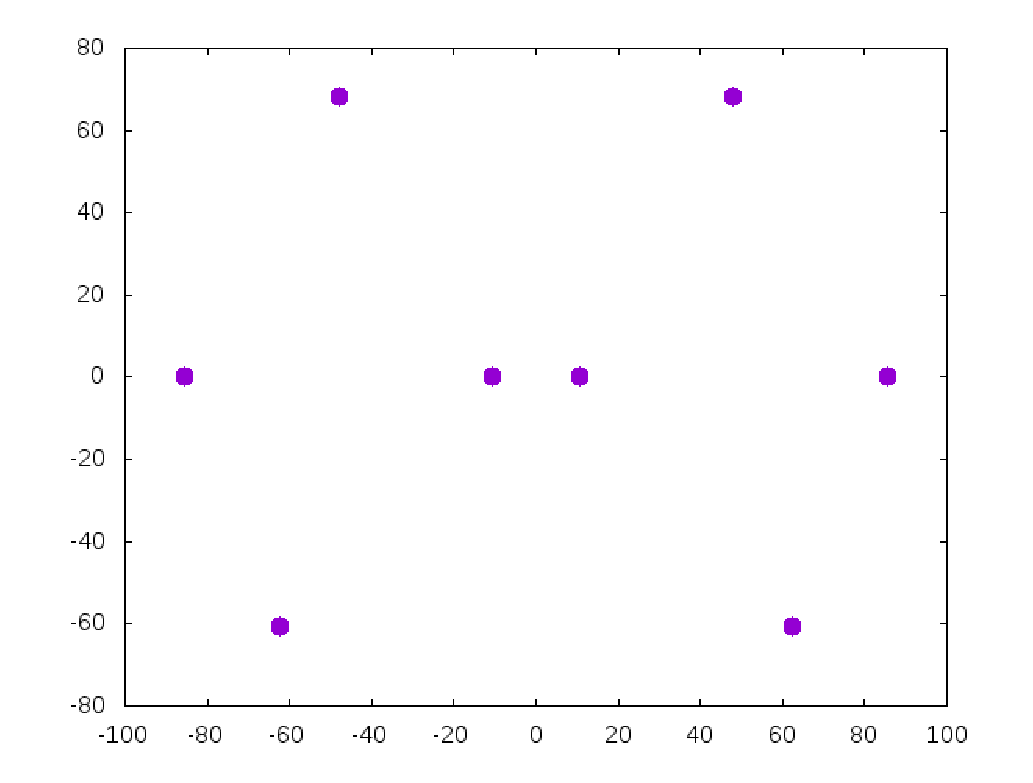
\includegraphics[width=.48\linewidth]{Avdeev_8_171_1538491142044.eps}
	\\
	\parbox{.48\linewidth}{\caption{}\label{Avdeev_8_168_1538490487450.eps}}
	\hfill
	\parbox{.48\linewidth}{\caption{}\label{Avdeev_8_171_1538491142044.eps}}
\end{figure}









\begin{figure}[htbp]
	\includegraphics[width=.48\linewidth]{Avdeev_9_123_1538485102263.eps}
	\hfill
	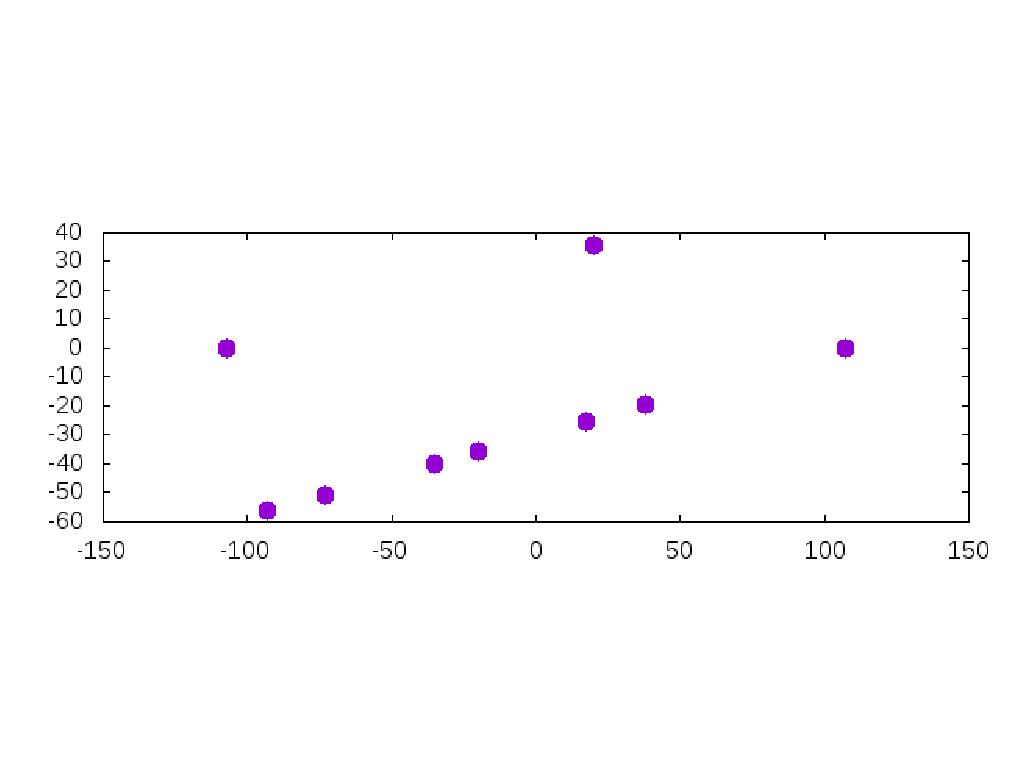
\includegraphics[width=.48\linewidth]{Avdeev_9_214_1538495187150.eps}
	\\
	\parbox{.48\linewidth}{\caption{}\label{Avdeev_9_123_1538485102263.eps}}
	\hfill
	\parbox{.48\linewidth}{\caption{}\label{Avdeev_9_214_1538495187150.eps}}
\end{figure}





\begin{figure}[htbp]
	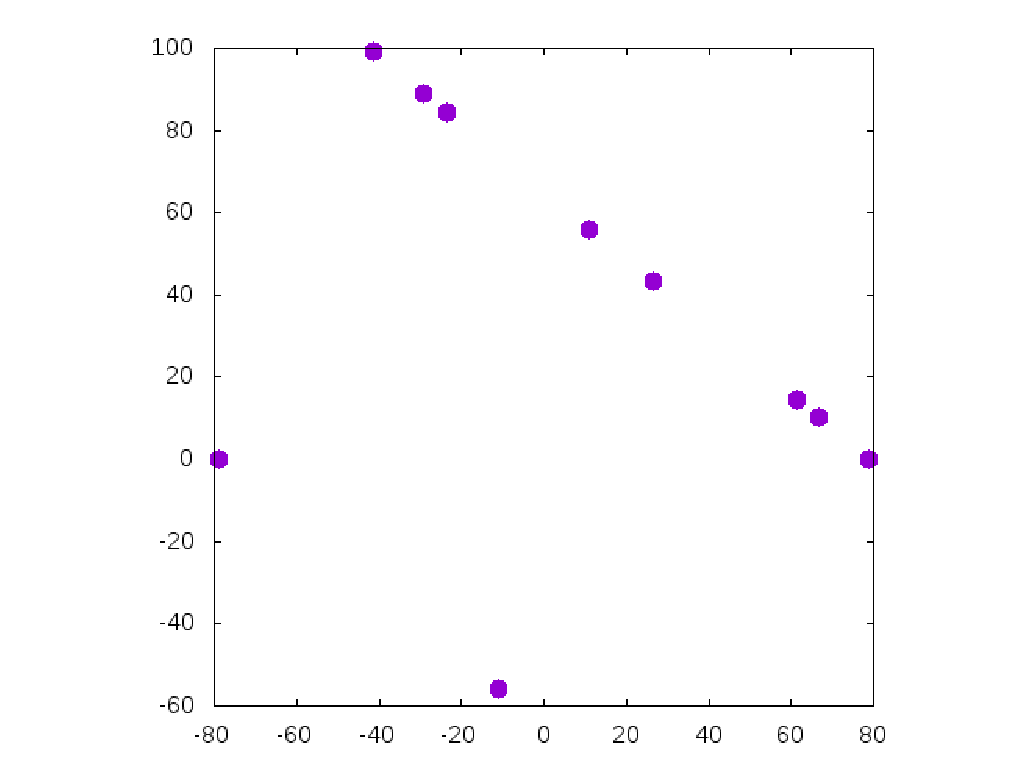
\includegraphics[width=.48\linewidth]{Avdeev_10_158_1538485325776.eps}
	\hfill
	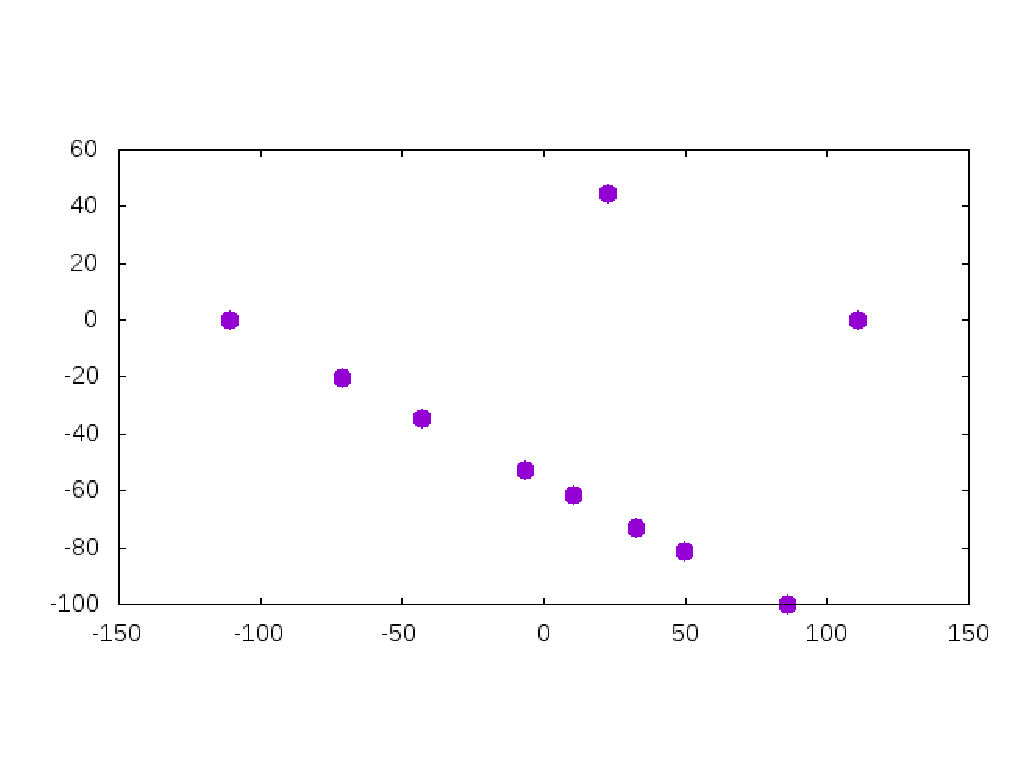
\includegraphics[width=.48\linewidth]{Avdeev_10_222_1538488624864.eps}
	\\
	\parbox{.48\linewidth}{\caption{}\label{F1}}
	\hfill
	\parbox{.48\linewidth}{\caption{}\label{F2}}
\end{figure}

\end{itemize}


\bigskip\centerline{\bf Литература}


1.	\emph{Инфантьева А.~С., Катышев П.~А.} Тематическая организация Интернет-эгоистории в ранговом распределении Ципфа / А.~С.~Инфантьева, П.~А.~Катышев; Вестник Кемеровского государственного университета. – 2012. – №. 1. (49). С. 160-163.

2.	\emph{Авдеев Н.~Н.} Программа анализа грамотности интер\-нет\--СМИ // Культура общения и её формирование. – 2016. – С. 81-83.


3.	\emph{ Авдеев Н.~Н., Шевелева К.~В.} Анализ орфографической грамотности
математических образовательных ресурсов в сети «Интернет» // Некоторые вопросы анализа, алгебры, геометрии и математического
образования – Воронеж: Издательско-полиграфический центр «Научная книга», 2017. – Вып. 7, Часть I – 244 с.

4.	\emph{Авдеев Н.~Н., Шевелева К.~В.} Математическое моделирование распространённых орфографических ошибок с помощью регулярных выражений на материале математических образовательных ресурсов в сети «Интернет» // Материалы международной конференции  «Воронежская зимняя математическая школа С. Г. Крейна – 2018» [Текст] / под ред. В. А. Костина. – Воронеж : Издательско-полиграфический центр «Научная книга», 2018. –  С.110-112

5.	\emph{Sheveleva K.~V.} Elementary generalization of Zipf's law for spelling mistakes (based on internet resources devoted to mathematics)  / K.~V.~Sheveleva// «Вестник современных исследований»  Выпуск № 8-3 (23) (август, 2018). --  Научный центр «Орка»,  Омск, 2018 -- C.362--363

6.	\emph{Маслов В. П., Маслова Т. В.} О законе Ципфа и ранговых распределениях в лингвистике и семиотике //Математические заметки. – 2006. – Т. 80. – №. 5. – С. 718-732.

7.  \emph{Ляпунов С.~М., Алымов А.~С.}  Методология анализа текста с помощью составления частотных словарей по частям речи //Научный альманах. – 2017. – №. 10-3. – С. 203-206.

8.	\emph{Кочеткова Н.~А., Клышинский Э.~С., Ермаков П.~Д.} Подчиняются ли составные конструкции закону Ципфа? //Системный администратор. – 2016. – №. 11. – С. 89-95.

9.  \emph{Чичкарёв Е.~А.} Компьютерная математика с Maxima: Руководство для школьников и студентов //М.: ALT Linux. – 2012. – Т. 384.

10. \emph{Алексеев Е.~Р., Чеснокова О.~В.} Введение в Octave для инженеров и математиков //М.: ALT Linux. – 2012.

11. \emph{Алексеев Е.~Р.} Использование свободных программ в научных исследованиях // Прикладная информатика. – 2009. – №. 6.



{\small Работа выполнена в Воронежском университете при поддержке РНФ, грант 16-11-10125.}


{\bf Авдеев Николай Николаевич},
бакалавр математики, магистрант кафедры функционального анализа и операторных уравнений математического факультета
ФГБОУ ВО <<Воронежский государственный университет>>, г. Воронеж.

E-mail: avdeev@math.vsu.ru, nickkolok@mail.ru

Научный руководитель: Семенов Евгений Михайлович.

\end{document}

